\section{Resultados e discussão}\label{sec:resultados}

Esta seção apresenta os resultados obtidos com o framework de otimização descrito na Seção~\ref{sec:metodologia}, aplicado a uma matriz de configurações de ponte de madeira roliça para estrada vicinal de pista simples.
A matriz combina quatro vãos teóricos com as cinco classes de resistência de madeiras de florestas nativas da \textcite{NBR7190-1:2022}, mantendo fixos a largura da pista, o trem tipo e todos os coeficientes normativos, de modo que as diferenças observadas decorram exclusivamente do vão e da classe de resistência.

A apresentação está organizada em quatro blocos.
O primeiro descreve o framework computacional desenvolvido (Seção~\ref{sec:plataforma}) e define a matriz de casos (Seção~\ref{sec:casos}).
O segundo detalha uma célula de referência da matriz (Seção~\ref{sec:caso_detalhado}), na qual são exercitados todos os recursos analíticos da ferramenta: convergência por hipervolume, fronteira eficiente, grau de utilização das verificações, custo da robustez, sensibilidade global de Sobol e dispersão das variáveis de projeto.
O terceiro percorre a matriz completa (Seção~\ref{sec:varredura}) e converte os resultados em ábacos de anteprojeto (Seção~\ref{sec:abacos}).
O quarto ajusta ao banco de dados da varredura uma equação fechada de pré-dimensionamento (Seção~\ref{sec:equacao}), alternativa numérica à leitura gráfica dos ábacos.


\subsection{Framework computacional}\label{sec:plataforma}

O framework de análise e otimização descrito na Seção~\ref{sec:metodologia} foi implementado em uma plataforma computacional de acesso livre para o dimensionamento de pontes de madeira, capaz de realizar a verificação completa dos elementos estruturais em conformidade com as \textcite{NBR7190-1:2022} e \textcite{nbr7188} \parencite{ReliaBridge2026}.
Para cada solução processada, a plataforma disponibiliza a fronteira eficiente, o memorial de verificação e as estatísticas descritivas das variáveis de projeto, servindo como instrumento de implementação e transferência dos resultados deste trabalho ao projetista.

\subsection{Definição da matriz de casos de estudo}\label{sec:casos}

Os parâmetros geométricos, de carregamento e os coeficientes normativos mantidos constantes em toda a matriz são apresentados na Tabela~\ref{tab:parametros}.
A largura de pista de 4{,}5~m corresponde à seção transversal usual de ponte vicinal de pista simples, compatível com o tráfego de um veículo por vez e com guarda-rodas laterais.

\begin{table}[!ht]
\caption{Parâmetros geométricos, de carregamento e coeficientes normativos comuns a toda a matriz.\label{tab:parametros}}
\begin{threeparttable}
\begin{tabular*}{\columnwidth}{@{\extracolsep\fill}lc@{\extracolsep\fill}}
\toprule
Parâmetro & Valor \\
\midrule
Largura da pista, $b_{w,\mathrm{pista}}$ (cm) & 450 \\
Trem tipo (ABNT NBR 7188) & TB-240 \\
Carga concentrada por roda, $p_{rodak}$ (kN) & 40 \\
Carga variável distribuída, $p_{qk}$ (kPa) & 4 \\
Carga permanente distribuída (rodeiro), $p_{gk}$ (kPa)\tnote{a} & 0{,}10 \\
Distância entre eixos, $a$ (m) & 1{,}5 \\
Classe de carregamento & Curta duração \\
Classe da madeira & Madeira natural \\
Classe de umidade & 3 \\
Coeficiente parcial das ações permanentes, $\gamma_g$ & 1{,}30 \\
Coeficiente parcial das ações variáveis, $\gamma_q$ & 1{,}50 \\
Coeficiente de minoração (tensões normais), $\gamma_{wf}$ & 1{,}40 \\
Coeficiente de minoração (cisalhamento), $\gamma_{wc}$ & 1{,}80 \\
Fator de combinação quase permanente, $\psi_2$ & 0{,}30 \\
Coeficiente de fluência, $\varphi$ & 0{,}80 \\
Desvio de robustez, $\rho$ (\%) & 5{,}0 \\
\bottomrule
\end{tabular*}
\begin{tablenotes}
\footnotesize
\item[a] O peso próprio do tabuleiro e das longarinas é calculado internamente pela plataforma a partir da geometria e da densidade da madeira. A carga permanente $p_{gk}$ representa apenas a ação sobreposta do rodeiro, isto é, das tábuas longitudinais de rolamento que guiam as rodas.
Estimou-se essa parcela a partir de duas tábuas de seção $5 \times 30$~cm, com densidade de 620~kg/m\textsuperscript{3} ($\gamma \approx 6{,}1$~kN/m\textsuperscript{3}), resultando em cerca de 0{,}18~kN/m ao longo do vão, ou aproximadamente 0{,}04~kPa quando distribuída sobre a largura da pista.
Adotou-se o valor de 0{,}10~kPa, arredondado para cobrir fixações e a maior densidade usual das peças de rolamento.
\item As propriedades mecânicas da madeira não constam desta tabela por variarem entre as células da matriz. São as da Tabela~\ref{tab:classes_madeira}, conforme a classe de resistência de cada célula.
\end{tablenotes}
\end{threeparttable}
\end{table}

A matriz de casos é o produto cartesiano de quatro vãos teóricos por cinco classes de resistência, totalizando vinte configurações, conforme a Tabela~\ref{tab:matriz}.
A faixa de vãos de 3{,}0 a 6{,}0~m foi escolhida por dois motivos.
O primeiro é de representatividade: corresponde à extensão usual dos cursos d'água transpostos por pontes de madeira roliça em vias vicinais.
O segundo é de consistência de formulação: nesse intervalo o momento fletor devido à carga móvel é dado integralmente pela Equação~\eqref{eq:mqk30}, sem a parcela adicional de multidão da Equação~\eqref{eq:mqk45}, de modo que as curvas de resultado não apresentam descontinuidade de formulação.

\begin{table}[!ht]
\caption{Matriz de casos de estudo. Cada célula corresponde a uma execução independente do NSGA-II.\label{tab:matriz}}
\begin{threeparttable}
\begin{tabular*}{\columnwidth}{@{\extracolsep\fill}lccccc@{\extracolsep\fill}}
\toprule
 & \multicolumn{5}{c}{Classe de resistência (ABNT NBR 7190-3)} \\
\cmidrule{2-6}
Vão $L$ (m) & D20 & D30 & D40 & D50 & D60 \\
\midrule
3{,}0 & C-01 & C-02 & C-03 & C-04 & C-05 \\
4{,}0 & C-06 & C-07 & C-08 & C-09 & C-10 \\
5{,}0 & C-11 & C-12 & \textbf{C-13} & C-14 & C-15 \\
6{,}0 & C-16 & C-17 & C-18 & C-19 & C-20 \\
\bottomrule
\end{tabular*}
\begin{tablenotes}
\footnotesize
\item A célula C-13 ($L = 5{,}0$~m, classe D40), destacada em negrito, é adotada como caso de referência para a análise detalhada da Seção~\ref{sec:caso_detalhado}.
\end{tablenotes}
\end{threeparttable}
\end{table}

Os intervalos de busca das cinco variáveis de projeto, comuns a todas as células, são apresentados na Tabela~\ref{tab:intervalos}.
Os limites foram estabelecidos de modo a abranger as dimensões comerciais usuais de madeira roliça e de pranchas serradas, sem restringir artificialmente o espaço de busca do algoritmo.

\begin{table}[!ht]
\caption{Intervalos adotados para as variáveis de projeto.\label{tab:intervalos}}
\begin{threeparttable}
\begin{tabular*}{\columnwidth}{@{\extracolsep\fill}lcc@{\extracolsep\fill}}
\toprule
Variável & Valor mínimo (cm) & Valor máximo (cm) \\
\midrule
Diâmetro da longarina, $d$ & 20 & 100 \\
Largura da prancha do tabuleiro, $b_w$ & 20 & 50 \\
Altura da prancha do tabuleiro, $h$ & 5 & 15 \\
Espaçamento entre longarinas, $esp_{long}$ & 30 & 200 \\
Espaçamento entre peças do tabuleiro, $esp_{tab}$ & 2 & 5 \\
\bottomrule
\end{tabular*}
\end{threeparttable}
\end{table}

\subsection{Caso de referência detalhado: $L = 5{,}0$~m, classe D40}\label{sec:caso_detalhado}

Esta seção exercita todos os recursos analíticos da plataforma sobre uma única célula da matriz, a C-13.
A escolha recai sobre um vão intermediário e uma classe de resistência intermediária, de modo que o comportamento observado seja representativo do conjunto.
Os resultados das demais dezenove células são reportados de forma condensada na Seção~\ref{sec:varredura}.

\subsubsection{Convergência da otimização}\label{sec:hipervolume}

A qualidade de uma fronteira aproximada é avaliada, de forma independente da inspeção visual, pelo indicador de hipervolume ($HV$), que mede a fração do espaço objetivo dominada pela fronteira em relação a um ponto de referência $\mathbf{r}$, conforme a Equação~\eqref{eq:hv} \parencite{blank2020}.

\begin{equation}
HV(\mathcal{F}_1, \mathbf{r}) = \mathrm{Vol}\left(\bigcup_{\mathbf{x} \in \mathcal{F}_1} \left[f_1(\mathbf{x}), r_1\right] \times \left[f_2(\mathbf{x}), r_2\right]\right)
\label{eq:hv}
\end{equation}

Os objetivos são normalizados pelos pontos ideal e nadir observados ao longo de toda a execução, de modo que o indicador resulte adimensional e comparável entre células de escalas distintas, e adota-se o ponto de referência $r_1 = r_2 = 1{,}1$ nesse espaço normalizado.
A Figura~\ref{fig:convergencia_hv} apresenta a evolução do hipervolume em função do número de gerações para a célula C-13.

\begin{figure}[!ht]
    \centering
    
\includegraphics[width=0.45\textwidth]{figuras/en/convergencia_hv.png}
    \caption{Evolução do hipervolume ao longo das gerações do NSGA-II.}
    \label{fig:convergencia_hv}
\end{figure}

A curva apresenta crescimento acentuado nas primeiras vinte gerações e refinamento assintótico depois disso, com estabilização na geração 40, o que confirma a convergência da otimização com o número de gerações adotado na Tabela~\ref{tab:nsga2}.
Nas vinte células da matriz, a estabilização ocorre entre as gerações 21 e 153, sempre antes das 300 gerações executadas.
O \textit{spacing} da fronteira, que mede a variação da distância entre soluções vizinhas, foi baixo em toda a matriz, entre 0{,}0136 e 0{,}0203, o que garante a uniformidade da distribuição das soluções obtidas ao longo da fronteira.

\subsubsection{Fronteira eficiente e soluções representativas}\label{sec:fronteira_ref}

A otimização robusta multiobjetivo da célula C-13, com $\rho = 5\%$, gerou um conjunto de soluções não dominadas distribuídas ao longo da fronteira eficiente, apresentada na Figura~\ref{fig:fronteira_ref}.
A Tabela~\ref{tab:solucoes_ref} reúne uma amostra representativa dessas soluções, com as respectivas funções objetivo e o maior valor entre as seis funções limite, confirmando o atendimento aos critérios normativos mesmo sob a avaliação robusta.

\begin{figure}[!ht]
    \centering
    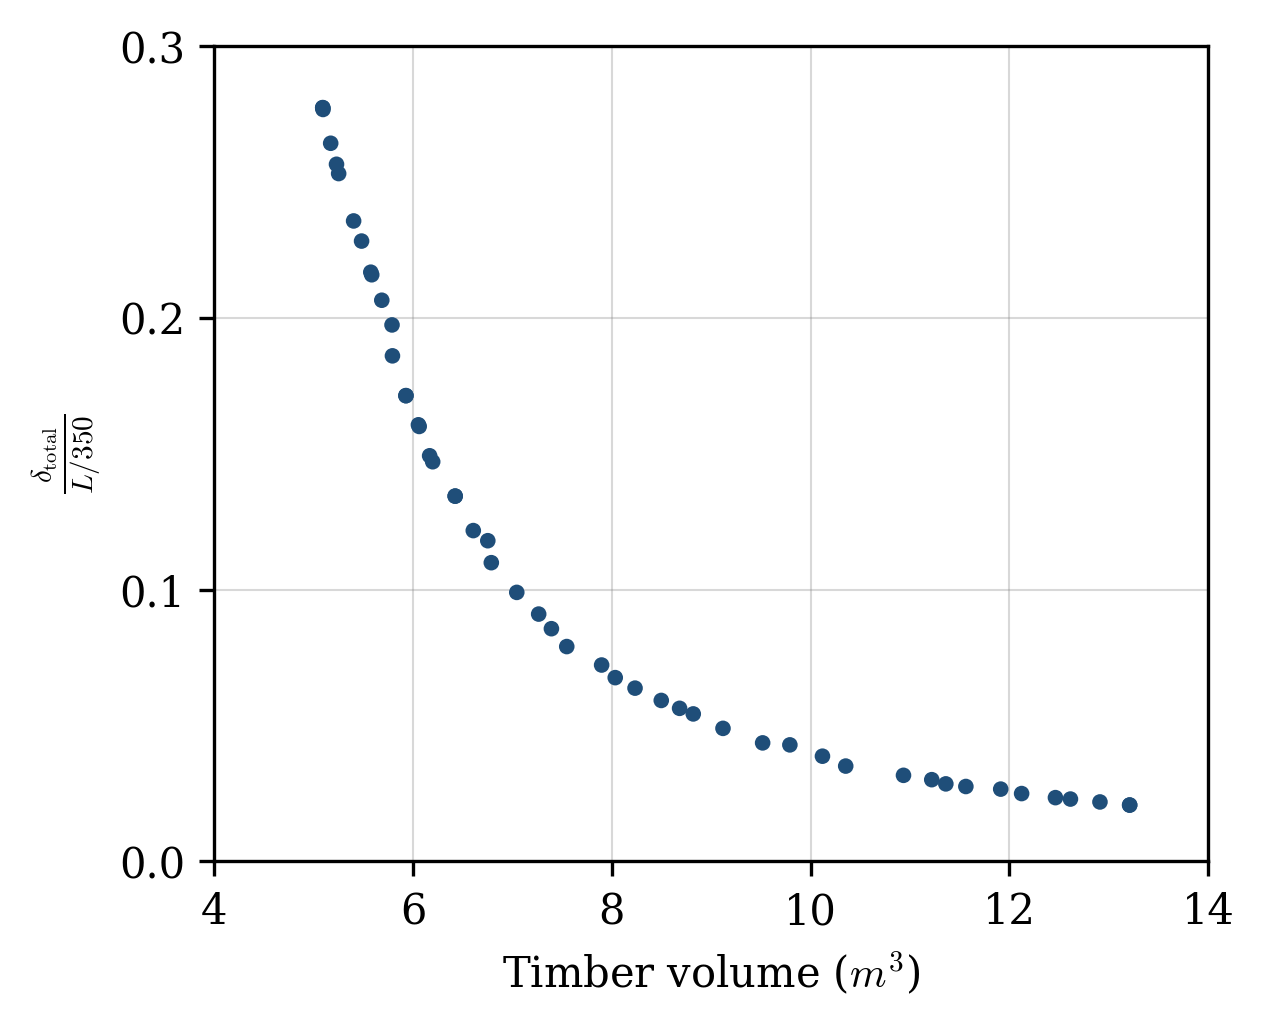
\includegraphics[width=0.6\textwidth]{figuras/en/pareto_frontier_C13.png}
    \caption{Fronteira eficiente da célula de referência C-13 ($L = 5{,}0$~m, D40, $\rho = 5\%$).}
    \label{fig:fronteira_ref}
\end{figure}

\begin{table}[!ht]
\caption{Soluções representativas da fronteira eficiente da célula C-13.\label{tab:solucoes_ref}}
\begin{threeparttable}
\setlength{\tabcolsep}{3pt}
\begin{tabular*}{\textwidth}{@{\extracolsep{\fill}}cccccccc@{\extracolsep{\fill}}}
\toprule
$d$ (cm) & $b_w$ (cm) & $h$ (cm) & $esp_{long}$ (cm) & $esp_{tab}$ (cm) & $V_{\mathrm{total}}$ (m\textsuperscript{3}) & $\delta_{\mathrm{tot}}/(L/350)$ & $g_{\max}$ \\
\midrule
47{,}78 & 45{,}51 & 7{,}34 & 69{,}98 & 2{,}24 & 5{,}09 & 0{,}2772 & $-0{,}0018$ \\
51{,}01 & 45{,}50 & 7{,}26 & 67{,}89 & 4{,}73 & 5{,}57 & 0{,}2167 & $-0{,}0431$ \\
56{,}41 & 45{,}50 & 11{,}29 & 110{,}54 & 4{,}69 & 6{,}06 & 0{,}1600 & $-0{,}0012$ \\
64{,}15 & 45{,}55 & 10{,}71 & 97{,}85 & 4{,}98 & 7{,}04 & 0{,}0990 & $-0{,}0471$ \\
75{,}71 & 45{,}50 & 10{,}09 & 92{,}98 & 2{,}55 & 8{,}82 & 0{,}0543 & $-0{,}0759$ \\
90{,}92 & 45{,}50 & 7{,}93 & 58{,}55 & 2{,}57 & 11{,}36 & 0{,}0285 & $-0{,}0959$ \\
100{,}00 & 45{,}50 & 6{,}99 & 81{,}23 & 4{,}53 & 13{,}21 & 0{,}0208 & $-0{,}0002$ \\
\bottomrule
\end{tabular*}
\begin{tablenotes}
\footnotesize
\item Sete soluções extraídas da fronteira final de 50 pontos não dominados, ordenadas do extremo de menor volume de madeira (primeira linha) ao extremo de menor flecha adimensional (última linha), incluindo ambos os extremos. $g_{\max}$ é o maior valor entre as funções limite de resistência e de serviço $g_1$ a $g_4$ da solução, e é negativo em todas as linhas, o que confirma a viabilidade sob a avaliação robusta.
As funções limite geométricas $g_5$ e $g_6$, que apenas verificam o enquadramento dos espaçamentos nos intervalos da Tabela~\ref{tab:intervalos}, não entram nesse máximo por não expressarem margem estrutural.
\end{tablenotes}
\end{threeparttable}
\end{table}

A fronteira estende-se de 5{,}09~m\textsuperscript{3} de madeira, com flecha total igual a 27{,}7\% do limite normativo, até 13{,}21~m\textsuperscript{3}, com flecha de apenas 2{,}1\% do limite.
Os dois objetivos variam, portanto, em escalas distintas. O volume pouco mais que duplica (2{,}6 vezes), enquanto a flecha adimensional cai cerca de treze vezes.
Esse desequilíbrio é a manifestação direta da geometria da seção circular.
O volume cresce aproximadamente com $d^{1{,}28}$ ao longo da fronteira, ao passo que a flecha decresce com $d^{-3{,}54}$, de modo que o ajuste conjunto resulta em $\delta_{\mathrm{tot}}/(L/350) \propto V^{-2{,}76}$, com coeficiente de determinação de 0{,}995.
Em termos de projeto, isso significa que os primeiros metros cúbicos adicionais de madeira compram uma redução expressiva de deslocamento. Dobrar o volume a partir do extremo econômico já reduz a flecha em cerca de sete vezes, e dobrá-lo novamente reduziria esse valor por um fator adicional semelhante, ainda que a fronteira estudada não chegue a cobrir essa segunda duplicação.

O trecho útil da fronteira para o projetista concentra-se, assim, na primeira metade do intervalo de volumes. Já em 7{,}90~m\textsuperscript{3}, cerca de um terço do caminho entre os extremos, a flecha cai para 7{,}2\% do limite. Além desse ponto, o retorno marginal cai de $V = 8{,}82$~m\textsuperscript{3} para $V = 13{,}21$~m\textsuperscript{3} (acréscimo de 49{,}5\%), a flecha cai de apenas 5{,}4\% para 2{,}1\% do limite, um ganho de pouco mais de três pontos percentuais sobre uma margem já folgada. Aumentar o volume além do primeiro terço da fronteira, portanto, deixa de se justificar na prática.


A restrição ativa ao longo da fronteira é a mesma do início ao fim.
A flexão do tabuleiro ($g_4$) é a verificação mais próxima do limite nas 50 soluções da fronteira, sem exceção, inclusive no extremo de menor volume, onde satura praticamente no limite normativo ($g_{\max} \approx 0$, utilização de 99{,}8\%).
A flexão da longarina ($g_1$) acompanha de perto nesse mesmo extremo, com utilização de 99{,}7\%, mas não chega a ultrapassar o tabuleiro como restrição governante em nenhum ponto da fronteira nesta versão da matriz, o que ainda assim confirma o quão próximas as duas verificações permanecem uma da outra.
Portanto, é possível afirmar que percorrer a fronteira significa aumentar o diâmetro da longarina, que rapidamente ganha folga, ao passo que o tabuleiro permanece ancorado no seu limite ao longo de toda a extensão do espaço de compromisso.
O tabuleiro, portanto, não é um elemento secundário do dimensionamento e sim o elemento que limita o desempenho. O par largura-altura da prancha e o espaçamento entre longarinas definem o vão de flexão local sob a roda, e são eles que ditam a forma da curva da Figura~\ref{fig:fronteira_ref}.

\subsubsection{Grau de utilização das verificações normativas}\label{sec:utilizacao}

A Figura~\ref{fig:utilizacao} apresenta o grau de utilização de cada verificação normativa para uma solução selecionada da fronteira, entendido como a razão entre solicitação e resistência, no caso dos estados limites últimos, ou entre deslocamento e limite admissível, no caso do estado limite de serviço.
O valor de 100\% corresponde ao limite normativo.
Como as funções limite são normalizadas na forma $g_j = (S_j - R_j)/R_j$, o grau de utilização decorre diretamente delas por $(1 + g_j)\times 100\%$.
A solução analisada é a de menor volume de madeira da fronteira, primeira linha da Tabela~\ref{tab:solucoes_ref}, por ser a de interesse imediato para o anteprojeto.

\begin{figure}[!ht]
    \centering
    
\includegraphics[width=0.65\textwidth]{figuras/en/utilizacao_C13.png}
    \caption{Grau de utilização de cada verificação normativa para a solução selecionada da fronteira robusta da célula C-13.}
    \label{fig:utilizacao}
\end{figure}

A solução econômica da célula C-13 apresenta duas verificações praticamente saturadas e duas com folga relevante.
A flexão do tabuleiro governa o dimensionamento, com utilização de 99{,}8\%, valor consistente com o $g_{\max} \approx 0$ registrado na primeira linha da Tabela~\ref{tab:solucoes_ref}.
Imediatamente atrás vem a flexão da longarina, a 99{,}7\%.
As duas verificações de flexão, portanto, tornam-se ativas quase simultaneamente, o que é a assinatura de um dimensionamento bem equilibrado: o algoritmo não pôde reduzir mais o volume porque teria de violar uma das duas ao mesmo tempo em que a outra ainda estava no limite.

As folgas concentram-se nas verificações restantes, embora de forma desigual entre elas.
A flecha da longarina ($g_3$, que combina os limites $L/350$ quase permanente e $L/500$ raro) opera a 77{,}7\% do seu limite combinado, e o cisalhamento a apenas 44{,}9\% da resistência de cálculo, sendo esta última a verificação com maior reserva.

No vão de 5~m, para a madeira D40 e o trem tipo TB-240, o dimensionamento continua controlado por resistência à flexão, e não por rigidez, mas a folga de deslocamento já não é tão ampla quanto a das demais células. A Seção~\ref{sec:varredura} mostra que, em classes ainda mais rígidas no mesmo vão ou em vãos maiores, essa mesma verificação chega a governar.
A ampla folga ao cisalhamento decorre da geometria circular, na qual a área da seção cresce com $d^2$ enquanto a solicitação de cortante independe do diâmetro, e indica que a verificação ao esforço cortante, tradicionalmente citada como crítica em peças roliças curtas, não é determinante nesta faixa de vãos.


\subsubsection{Custo da robustez}\label{sec:custo_robustez}

A otimização determinística tende a posicionar as soluções ótimas exatamente sobre a fronteira das restrições ativas, tornando-as sensíveis a pequenas variações nas variáveis de projeto.
Em pontes de madeira roliça, essa sensibilidade é agravada pela variabilidade natural do diâmetro das peças e pelas tolerâncias de fabricação e montagem.
A incorporação da robustez desloca a fronteira eficiente para o interior do domínio viável, penalizando soluções com função limite de flexão da longarina praticamente nula ($g_1 \approx 0$), pois sob perturbação de $\pm\rho$ parte das realizações resultaria em violação.

Para quantificar esse efeito, a célula C-13 foi reotimizada para cinco níveis de desvio em grade uniforme, $\rho \in \{0\%,\ 5\%,\ 10\%,\ 15\%,\ 20\%\}$, mantendo inalterados todos os demais parâmetros do algoritmo (Tabela~\ref{tab:nsga2}).
O caso $\rho = 0\%$ corresponde à otimização determinística, com $N_c = 1$, e serve de referência.
A grade foi estendida até $\rho = 20\%$, bem além do valor de projeto de 5\% adotado no restante da matriz, para caracterizar a relação entre $\rho$ e o custo de volume ao longo de uma faixa mais ampla do que a estritamente necessária ao projeto.
A comparação é feita em um único ponto de cada fronteira, a solução de menor volume (o extremo de interesse imediato para o anteprojeto), e não por faixas pareadas de flecha adimensional, leitura descartada por ser sensível ao ruído de uma única execução independente do NSGA-II por nível de $\rho$.

\begin{figure}[!ht]
    \centering
    
\includegraphics[width=0.7\textwidth]{figuras/en/custo_robustez_C13.png}
    \caption{Fronteiras eficientes da célula C-13 para $\rho = 0\%$, $5\%$, $10\%$, $15\%$ e $20\%$.}
    \label{fig:custo_robustez}
\end{figure}

\begin{table}[!ht]
\caption{Volume mínimo da fronteira eficiente da célula C-13 para cada nível de desvio $\rho$, e acréscimo percentual em relação ao caso determinístico ($\rho = 0\%$).\label{tab:custo_robustez}}
\begin{threeparttable}
\begin{tabular*}{\columnwidth}{@{\extracolsep\fill}ccc@{\extracolsep\fill}}
\toprule
$\rho$ (\%) & $V_{\min}$ (m\textsuperscript{3}) & $\Delta$ \\
\midrule
0{,}0 & 4{,}800 & -- \\
5{,}0 & 5{,}090 & $+6{,}0\%$ \\
10{,}0 & 5{,}414 & $+12{,}8\%$ \\
15{,}0 & 5{,}788 & $+20{,}6\%$ \\
20{,}0 & 6{,}091 & $+26{,}9\%$ \\
\bottomrule
\end{tabular*}
\begin{tablenotes}
\footnotesize
\item $V_{\min}$ é o volume da solução de menor volume de madeira da fronteira eficiente naquele nível de $\rho$. $\Delta$ é o acréscimo percentual em relação a $V_{\min}(\rho{=}0\%)$.
\end{tablenotes}
\end{threeparttable}
\end{table}

A Figura~\ref{fig:custo_robustez} mostra as cinco fronteiras deslocando-se de forma visível e ordenada para o interior do domínio viável à medida que $\rho$ cresce.
No extremo de menor volume, a Tabela~\ref{tab:custo_robustez} mostra um acréscimo monotônico e aproximadamente proporcional a $\rho$, de 4{,}800~m\textsuperscript{3} no caso determinístico a 5{,}090~m\textsuperscript{3} ($+6{,}0\%$) em $\rho = 5\%$, 5{,}414~m\textsuperscript{3} ($+12{,}8\%$) em $\rho = 10\%$, 5{,}788~m\textsuperscript{3} ($+20{,}6\%$) em $\rho = 15\%$ e 6{,}091~m\textsuperscript{3} ($+26{,}9\%$) em $\rho = 20\%$.
A taxa marginal de custo cresce discretamente com $\rho$, de cerca de 1{,}2\% de volume adicional por ponto percentual de $\rho$ entre 0 e 5\%, a cerca de 1{,}3\% a 1{,}4\% por ponto percentual nos níveis mais altos da grade.

O valor $\rho = 5\%$ permanece adotado como padrão em toda a matriz (Seção~\ref{sec:varredura}) por consistência com a literatura sobre tolerâncias dimensionais de peças roliças.

\subsubsection{Análise de sensibilidade global por índices de Sobol}\label{sec:sobol}

Para identificar quais variáveis de projeto mais influenciam a violação de cada restrição sob perturbação, realizou-se uma análise de sensibilidade global pelo método de Sobol \parencite{Sobol2001}, implementado na biblioteca \texttt{UQpy} \parencite{Olivier2020}.
Os índices de efeito total $S_{T_i}$ das cinco variáveis de projeto foram estimados em relação às seis funções limite, a partir de uma amostragem independente de $N = 20\,000$ pontos no domínio de cada variável (Tabela~\ref{tab:intervalos}).

\begin{figure}[!ht]
    \centering
    
\includegraphics[width=0.85\textwidth]{figuras/en/sobol_heatmap_C13.png}
    \caption{Índices de Sobol de efeito total ($S_{T_i}$) das variáveis de projeto sobre as restrições, célula C-13.}
    \label{fig:sobol}
\end{figure}

\begin{table}[!ht]
\caption{Variável de maior influência ($S_{T_i}$ dominante) por restrição.\label{tab:sobol}}
\begin{threeparttable}
\footnotesize
\setlength{\tabcolsep}{3pt}
\begin{tabular*}{\columnwidth}{@{\extracolsep\fill}lccc@{\extracolsep\fill}}
\toprule
Restrição & Variável dominante & $S_{T_i}$ & Participação \\
\midrule
$g_1$: flexão da longarina & $d$ & 1{,}005 & 98{,}2\% \\
$g_2$: cisalhamento da longarina & $d$ & 1{,}021 & 96{,}0\% \\
$g_3$: flecha da longarina & $d$ & 1{,}003 & 97{,}2\% \\
$g_4$: flexão do tabuleiro & $esp_{long}$ & 4{,}964 & 93{,}0\% \\
$g_5$: espaçamento entre longarinas & $esp_{long}$ & 1{,}003 & 100{,}0\% \\
$g_6$: espaçamento entre peças do tabuleiro & $esp_{tab}$ & 1{,}000 & 100{,}0\% \\
\bottomrule
\end{tabular*}
\begin{tablenotes}
\footnotesize
\item A participação relativa é a fração do somatório dos índices de efeito total das cinco variáveis para aquela restrição, calculada após truncar em zero as estimativas negativas.
Os índices de efeito total são estimados por diferença de variâncias e, por isso, não são limitados ao intervalo $[0,1]$ em respostas fortemente não lineares: o valor de 4{,}964 associado a $g_4$ reflete a não linearidade do arredondamento do número inteiro de peças acomodadas na pista.
\end{tablenotes}
\end{threeparttable}
\end{table}

O resultado confirma a expectativa mecânica para as três restrições da longarina.
O diâmetro $d$ responde por 98{,}2\% da sensibilidade da flexão, 96{,}0\% do cisalhamento e 97{,}2\% da flecha, ao passo que as quatro variáveis restantes somam, em conjunto, menos de 4\% em qualquer uma delas.
O domínio é esperado porque $d$ é a única variável que entra simultaneamente na área, no módulo resistente e no momento de inércia da seção circular, e é ainda mais pronunciado no estado limite de serviço, no qual o momento de inércia varia com $d^4$ enquanto a área, que governa o peso próprio, varia apenas com $d^2$.

A flexão do tabuleiro comporta-se de modo distinto e mais informativo.
Nela, o diâmetro é praticamente irrelevante, com participação de 0{,}1\%, e a variável dominante passa a ser o espaçamento entre longarinas, com 93{,}0\%, seguido pela altura da prancha, com 4{,}4\%, e pela largura, com 2{,}5\%.
O espaçamento entre longarinas é o vão de flexão local da prancha, nesta peça o momento solicitante cresce com o quadrado desse vão, ao passo que a resistência da mesma cresce apenas com $b_w h^2$.
O espaçamento entre longarinas é, portanto, a variável de acoplamento entre os dois subsistemas da superestrutura. Ela não afeta a longarina isoladamente, mas define quanto do carregamento chega a cada uma e qual o vão que o tabuleiro precisa vencer.
As duas últimas restrições são, por construção, funções exclusivas dos respectivos espaçamentos, e a análise as recupera com participação de 100\%, o que serve como verificação de consistência do próprio estimador.

Aqui é possível perceber uma hierarquia para eventuais controles de execução em pontes de madeira.
O diâmetro das peças roliças e o espaçamento entre longarinas concentram praticamente toda a sensibilidade do conjunto.
São elas que justificam investimento em controle dimensional rigoroso, o primeiro na etapa de seleção e classificação das toras, com rejeição das peças fora da faixa nominal, e o segundo na etapa de montagem, com gabarito de posicionamento das longarinas.
As dimensões da prancha do tabuleiro, $b_w$ e $h$, e o espaçamento entre peças do tabuleiro, $esp_{tab}$, admitem tolerâncias de execução mais folgadas sem prejuízo mensurável à segurança, uma vez que respondem por parcela reduzida da variabilidade das funções limite.
Essa distinção é relevante em obra vicinal, na qual o controle de qualidade é necessariamente seletivo e precisa ser direcionado ao que efetivamente importa.

\subsubsection{Dispersão das variáveis de projeto ao longo da fronteira}\label{sec:dispersao}

Como complemento aos indicadores de qualidade da fronteira no espaço objetivo, a Figura~\ref{fig:boxplot} caracteriza a diversidade da fronteira no espaço de decisão, apresentando a dispersão de cada variável de projeto entre as soluções não dominadas.

\begin{figure}[!ht]
    \centering
    
\includegraphics[width=0.75\textwidth]{figuras/en/boxplot_variaveis_C13.png}
    \caption{Dispersão das variáveis de projeto ao longo da fronteira eficiente da célula C-13.}
    \label{fig:boxplot}
\end{figure}

\begin{table}[!ht]
\caption{Estatística descritiva das variáveis de projeto na fronteira eficiente da célula C-13.\label{tab:estatistica}}
\begin{threeparttable}
\footnotesize
\setlength{\tabcolsep}{3pt}
\begin{tabular*}{\textwidth}{@{\extracolsep{\fill}}lccccccccc@{\extracolsep{\fill}}}
\toprule
Variável & Média & Desv. padrão & CV (\%) & Mínimo & $Q_1$ & Mediana & $Q_3$ & Máximo & Amplitude \\
\midrule
$d$ (cm) & 68{,}84 & 17{,}14 & 24{,}90 & 47{,}78 & 54{,}49 & 64{,}89 & 82{,}72 & 100{,}00 & 52{,}22 \\
$b_w$ (cm) & 45{,}58 & 0{,}20 & 0{,}44 & 45{,}50 & 45{,}50 & 45{,}50 & 45{,}51 & 46{,}60 & 1{,}10 \\
$h$ (cm) & 9{,}13 & 1{,}64 & 17{,}92 & 6{,}99 & 7{,}34 & 9{,}36 & 10{,}68 & 11{,}39 & 4{,}40 \\
$esp_{long}$ (cm) & 87{,}64 & 17{,}90 & 20{,}43 & 58{,}55 & 69{,}50 & 91{,}99 & 103{,}23 & 120{,}72 & 62{,}17 \\
$esp_{tab}$ (cm) & 3{,}44 & 1{,}14 & 33{,}14 & 2{,}18 & 2{,}44 & 2{,}56 & 4{,}68 & 4{,}98 & 2{,}79 \\
\bottomrule
\end{tabular*}
\begin{tablenotes}
\footnotesize
\item Estatísticas calculadas sobre as 50 soluções não dominadas da fronteira final.
\end{tablenotes}
\end{threeparttable}
\end{table}

A dispersão é fortemente desigual entre as variáveis, tanto em amplitude absoluta quanto em variação relativa.
O espaçamento entre longarinas é, com folga, a variável de maior amplitude ao longo da fronteira: 62{,}2~cm de variação, coeficiente de variação de 20{,}4\% e intervalo interquartil de 33{,}7~cm, cobrindo boa parte do domínio de busca da Tabela~\ref{tab:intervalos}.
Em seguida vem o diâmetro da longarina, com amplitude de 52{,}2~cm e coeficiente de variação de 24{,}9\%.
São essas duas variáveis, mesmo assim, que constroem o compromisso entre os dois objetivos: nenhuma outra se aproxima delas em amplitude absoluta.

No extremo oposto, a largura da prancha do tabuleiro é praticamente invariante, com coeficiente de variação de 0{,}4\% e intervalo interquartil de apenas 0{,}01~cm em torno de 45{,}5~cm.
O algoritmo converge para esse valor independentemente do ponto da fronteira escolhido pelo projetista, o que tem uma consequência prática direta: $b_w \approx 45{,}5$~cm pode ser fixado a priori no anteprojeto, sem penalidade de desempenho, reduzindo de cinco para quatro a dimensionalidade efetiva da decisão.
As duas variáveis restantes ocupam posições intermediárias, mas com leitura distinta entre si. A altura da prancha tem coeficiente de variação de 17{,}9\% (4{,}4~cm de amplitude), moderado, enquanto o espaçamento entre peças do tabuleiro tem 33{,}1\% (2{,}8~cm de amplitude), bem mais disperso, aproximando-se do mínimo admissível de 2~cm em pelo menos um ponto da fronteira (mínimo observado de 2{,}18~cm, a apenas 0{,}18~cm do piso do domínio de busca).

O confronto com a Seção~\ref{sec:sobol} é convergente.
As duas variáveis de maior sensibilidade são exatamente as duas de maior amplitude absoluta na fronteira, e cada uma comanda um subsistema, ainda que a ordem entre elas se inverta conforme o indicador. O espaçamento entre longarinas é a variável de maior amplitude na fronteira e responde por 93{,}0\% da sensibilidade da flexão do tabuleiro, ao passo que o diâmetro, segundo em amplitude, responde por 96 a 98\% da sensibilidade das três verificações da longarina.
Percorrer a fronteira consiste, portanto, em ajustar simultaneamente esses dois parâmetros, um por subsistema.
As três variáveis restantes, que reúnem baixa sensibilidade e amplitude absoluta reduzida, comportam-se como parâmetros construtivos e não como variáveis de decisão. Isso sugere que um procedimento de anteprojeto simplificado poderia fixá-las e otimizar apenas $d$ e $esp_{long}$ sem perda relevante de qualidade.

\subsection{Varredura paramétrica: efeito do vão e da classe de resistência}\label{sec:varredura}

Esta seção reporta o resultado das vinte células da matriz.
Para cada célula, extraiu-se da fronteira eficiente a solução de menor volume de madeira, por ser a de interesse imediato para o anteprojeto, e registraram-se as dimensões correspondentes, o volume total, a flecha adimensional e a verificação governante.
Os resultados consolidados constam da Tabela~\ref{tab:resultados_matriz}.

\begin{table}[!ht]
\caption{Resultados consolidados da varredura paramétrica: solução de menor volume de madeira em cada célula da matriz.\label{tab:resultados_matriz}}
\begin{threeparttable}
\footnotesize
\setlength{\tabcolsep}{3pt}
\begin{tabular*}{\textwidth}{@{\extracolsep{\fill}}llrrrrrrrrl@{\extracolsep{\fill}}}
\toprule
Célula & $L$ (m) / Classe & $d$ & $b_w$ & $h$ & $esp_{long}$ & $esp_{tab}$ & $V_{\mathrm{total}}$ & $\delta_{\mathrm{tot}}/(L/350)$ & $g_{\max}$ & Verificação \\
 & & (cm) & (cm) & (cm) & (cm) & (cm) & (m\textsuperscript{3}) & & & governante \\
\midrule
C-01 & 3{,}0 / D20 & 43{,}30 & 38{,}59 & 6{,}41 & 49{,}35 & 4{,}24 & 2{,}988 & 0{,}0943 & $-0{,}0000$ & Flexão tab. \\
C-02 & 3{,}0 / D30 & 37{,}77 & 38{,}59 & 6{,}44 & 55{,}16 & 4{,}20 & 2{,}464 & 0{,}1364 & $-0{,}0000$ & Flexão tab. \\
C-03 & 3{,}0 / D40 & 34{,}50 & 39{,}44 & 6{,}05 & 59{,}94 & 4{,}92 & 2{,}154 & 0{,}1634 & $-0{,}0007$ & Flexão tab. \\
C-04 & 3{,}0 / D50 & 31{,}81 & 38{,}57 & 5{,}85 & 62{,}83 & 2{,}20 & 1{,}903 & 0{,}1992 & $-0{,}0000$ & Flexão long. \\
C-05 & 3{,}0 / D60 & 30{,}12 & 38{,}58 & 5{,}57 & 64{,}70 & 5{,}00 & 1{,}745 & 0{,}2121 & $-0{,}0140$ & Flexão tab. \\
\midrule
C-06 & 4{,}0 / D20 & 52{,}37 & 26{,}72 & 5{,}00 & 32{,}20 & 2{,}84 & 5{,}089 & 0{,}1355 & $-0{,}0008$ & Flexão long. \\
C-07 & 4{,}0 / D30 & 45{,}85 & 45{,}73 & 8{,}71 & 72{,}78 & 2{,}69 & 4{,}076 & 0{,}1988 & $-0{,}0000$ & Flexão tab. \\
C-08 & 4{,}0 / D40 & 43{,}05 & 40{,}00 & 8{,}43 & 75{,}64 & 4{,}81 & 3{,}695 & 0{,}2149 & $-0{,}0068$ & Flexão tab. \\
C-09 & 4{,}0 / D50 & 38{,}71 & 35{,}69 & 5{,}04 & 54{,}90 & 4{,}81 & 3{,}163 & 0{,}2775 & $-0{,}0003$ & Flexão tab. \\
C-10 & 4{,}0 / D60 & 36{,}47 & 45{,}65 & 7{,}14 & 112{,}05 & 4{,}09 & 2{,}845 & 0{,}3132 & $-0{,}0004$ & Flexão tab. \\
\midrule
C-11 & 5{,}0 / D20 & 60{,}13 & 45{,}51 & 8{,}07 & 54{,}32 & 4{,}23 & 7{,}331 & 0{,}1585 & $-0{,}0005$ & Flexão long. \\
C-12 & 5{,}0 / D30 & 52{,}55 & 40{,}91 & 8{,}21 & 63{,}90 & 3{,}19 & 6{,}001 & 0{,}2277 & $-0{,}0001$ & Flexão tab. \\
\textbf{C-13} & 5{,}0 / D40 & 47{,}78 & 45{,}51 & 7{,}34 & 69{,}98 & 2{,}24 & 5{,}090 & 0{,}2772 & $-0{,}0018$ & Flexão tab. \\
C-14 & 5{,}0 / D50 & 44{,}49 & 45{,}50 & 10{,}89 & 125{,}17 & 4{,}61 & 4{,}562 & 0{,}3543 & $-0{,}0004$ & Flexão long. \\
C-15 & 5{,}0 / D60 & 41{,}79 & 45{,}50 & 6{,}55 & 78{,}07 & 3{,}01 & 4{,}084 & 0{,}3581 & $-0{,}0011$ & Flexão tab. \\
\midrule
C-16 & 6{,}0 / D20 & 66{,}72 & 45{,}42 & 6{,}47 & 38{,}08 & 2{,}11 & 9{,}978 & 0{,}1740 & $-0{,}0002$ & Flexão tab. \\
C-17 & 6{,}0 / D30 & 58{,}17 & 45{,}42 & 12{,}74 & 106{,}87 & 4{,}84 & 7{,}907 & 0{,}2718 & $-0{,}0015$ & Flexão long. \\
C-18 & 6{,}0 / D40 & 52{,}89 & 45{,}42 & 11{,}48 & 114{,}21 & 4{,}96 & 6{,}771 & 0{,}3333 & $-0{,}0003$ & Flexão tab. \\
C-19 & 6{,}0 / D50 & 49{,}24 & 45{,}43 & 10{,}55 & 119{,}44 & 2{,}45 & 6{,}015 & 0{,}3924 & $-0{,}0008$ & Flexão tab. \\
C-20 & 6{,}0 / D60 & 47{,}60 & 45{,}44 & 9{,}90 & 172{,}14 & 2{,}53 & 5{,}632 & 0{,}3914 & $-0{,}0000$ & Flexão tab. \\
\bottomrule
\end{tabular*}
\begin{tablenotes}
\footnotesize
\item Todas as células com $\rho = 5\%$ e os parâmetros de algoritmo da Tabela~\ref{tab:nsga2}.
A coluna ``Verificação governante'' registra a restrição com maior valor de $g_j$ entre $g_1$ e $g_4$ na solução reportada, isto é, a que está mais próxima do limite normativo, e $g_{\max}$ é o valor correspondente.
\end{tablenotes}
\end{threeparttable}
\end{table}

\paragraph{Efeito do vão.} O consumo de madeira cresce de forma mais que proporcional ao vão em todas as classes, como esperado, e o expoente da lei de potência $V \propto L^{n}$ ajustada às quatro observações de cada classe varia pouco entre classes, entre $n = 1{,}64$ (D40) e $n = 1{,}73$ (D20), com coeficientes de determinação de pelo menos 0{,}996 em todos os casos.
A tendência geral é de queda do expoente da D20 até a D40 ($n = 1{,}73$; 1{,}69; 1{,}64), seguida de recuperação parcial nas duas classes seguintes ($n = 1{,}67$ na D50 e $n = 1{,}68$ na D60), sem monotonicidade estrita ao longo da matriz.
Em termos absolutos, passar de 3{,}0 para 6{,}0~m multiplica o consumo por 3{,}3 na classe D20 e por 3{,}2 na classe D60, uma faixa bem mais estreita do que a observada entre as verificações governantes de cada classe permitiria supor.
O acoplamento entre peso próprio e desempenho, mais forte nas classes de menor resistência, segue presente como mecanismo, mas seu efeito sobre o expoente é discreto nesta faixa de vãos.

\paragraph{Efeito da classe de resistência.} A redução de volume ao subir de classe é, nesta matriz, aproximadamente uniforme entre os quatro vãos. Ao passar de D20 para D60, o consumo cai 41{,}6\% no vão de 3~m, 44{,}1\% no de 4~m, 44{,}3\% no de 5~m e 43{,}6\% no de 6~m.
Diferentemente do que uma matriz com domínio de busca mais restrito poderia sugerir, nenhuma das vinte células satura no piso dimensional de $d = 20$~cm da Tabela~\ref{tab:intervalos}. Mesmo a célula mais econômica, a C-05 (3~m, D60), converge para $d = 30{,}1$~cm, acima do piso.
A tabela revela, em vez disso, um padrão de convergência estrutural uniformemente apertada. Em todas as vinte células a solução de menor volume opera a no máximo 1{,}40\% de folga da verificação governante ($g_{\max}$ entre $-0{,}0140$ e $-0{,}0000$), sem folga relevante em nenhuma delas. A folga mais alta ocorre na C-05 (3~m, D60) e a segunda mais alta na C-08 (4~m, D40, $g_{\max} = -0{,}0068$), sem um padrão sistemático claro entre vão e margem.
Essa uniformidade é o resultado esperado de um algoritmo bem convergido explorando um domínio de busca contínuo, e substitui o efeito de saturação dimensional que uma faixa de diâmetros mais estreita produziria.

Em todos os vãos, o primeiro degrau de classe é o mais rentável, e por margem considerável.
Passar de D20 para D30 reduz o consumo entre 17{,}5\% (vão de 3~m) e 20{,}8\% (vão de 6~m), respondendo sozinho por 41\% a 48\% de toda a economia entre D20 e D60, ao passo que os degraus seguintes rendem, individualmente, entre 3{,}8\% e 12{,}4\% do volume de D20.
A causa do achatamento nos degraus seguintes é a compensação apontada na formulação do problema: entre D20 e D60 a resistência característica à flexão triplica e o módulo de elasticidade quase dobra, mas a densidade também dobra, de 500 para 1000~kg/m\textsuperscript{3}, e o acréscimo de peso próprio consome parte do ganho de resistência.
O ganho não chega a se anular nem a se inverter dentro da faixa estudada, de modo que não existe, a rigor, uma classe ótima no sentido de um mínimo interior.
Do ponto de vista de anteprojeto, a recomendação que decorre da matriz é que o esforço de especificação se concentre em garantir pelo menos a classe D30, em qualquer um dos quatro vãos, e que a busca por classes superiores só se justifique quando a madeira de classe alta estiver disponível sem sobrecusto relevante.

A matriz é integralmente monotônica, o que é a verificação de consistência esperada: dentro de cada classe o volume cresce com o vão, e dentro de cada vão decresce da classe D20 para a D60, sem uma única inversão nas vinte células.

\paragraph{Verificação governante.} A flexão domina integralmente a matriz. Quinze das vinte células são governadas pela flexão do tabuleiro e as cinco restantes pela flexão da longarina, sem nenhuma célula governada pela flecha.
As duas verificações de flexão alternam-se ao longo da matriz sem um padrão nítido em vão ou classe, coerente com o que a Seção~\ref{sec:fronteira_ref} mostra para a célula de referência.
A verificação de flecha da longarina ($g_3$), embora nunca governe, chega extremamente perto do limite em três células de vão e classe mais severos, com utilização de 99{,}21\% na C-15 ($L = 5{,}0$~m, D60), 99{,}90\% na C-19 ($L = 6{,}0$~m, D50) e 99{,}97\% na C-20 ($L = 6{,}0$~m, D60), sempre a poucos centésimos de ponto percentual atrás da flexão do tabuleiro.
O quase-empate mais estreito ocorre na C-20, em que a flexão do tabuleiro ($g_4 = -0{,}0000$, utilização de 100{,}00\%) e a flecha da longarina (99{,}97\%) diferem por menos de três centésimos de ponto percentual; a C-19 repete o padrão, com o tabuleiro a 99{,}92\% contra a flecha a 99{,}90\%, decidido pela quarta casa decimal.

A consequência prática permanece, em essência, a mesma, com uma ressalva relevante nas classes e vãos mais severos da matriz.
Em pontes de madeira roliça nesta faixa de vãos, sob o TB-240, a resistência à flexão governa a totalidade da matriz, e não a rigidez. O índice quase permanente $\delta_{\mathrm{tot}}/(L/350)$ permanece abaixo de 39{,}3\% em todas as vinte células (máximo de 0{,}392 na C-19).
A combinação rara ($L/500$, sem redução por fluência), contudo, já se aproxima do limite nas classes de maior resistência e vãos maiores, tornando-se quase ativa na C-15, na C-19 e na C-20, um alerta de que, para vãos ou classes além dos aqui estudados, a migração de resistência para rigidez pode ocorrer antes do que a leitura isolada do índice quase permanente sugeriria.

O cisalhamento, por sua vez, permanece longe do limite em toda a matriz, com utilização máxima de 60{,}2\%. A área da seção circular cresce com $d^2$ enquanto a solicitação de cortante independe do diâmetro, de modo que essa verificação, tradicionalmente citada como crítica em peças roliças curtas, não chega a se aproximar do limite mesmo após a correção da Equação~\eqref{eq:qqkenv} para vãos curtos.

\subsection{Ábacos de anteprojeto}\label{sec:abacos}

Os resultados da Tabela~\ref{tab:resultados_matriz} foram convertidos em ábacos de consulta direta, destinados ao uso do projetista na etapa de concepção, antes de qualquer processamento computacional.
A Figura~\ref{fig:abaco_volume} apresenta o volume total de madeira em função do vão, com uma curva por classe de resistência. A Figura~\ref{fig:abaco_volume_m2} normaliza esse volume pela área de tabuleiro, permitindo comparação direta entre vãos. Já a Figura~\ref{fig:abaco_diametro} fornece o diâmetro de longarina requerido, que é a informação de aquisição mais imediata para o projeto de engenharia.

\begin{figure}[!ht]
    \centering
    \begin{subfigure}{0.40\textwidth}
        \centering
        
\includegraphics[width=\textwidth]{figuras/en/abaco_volume_vs_vao.png}
        \caption{Volume total de madeira em função do vão teórico.}
        \label{fig:abaco_volume}
    \end{subfigure}
    \hfill
    \begin{subfigure}{0.40\textwidth}
        \centering
        
\includegraphics[width=\textwidth]{figuras/en/abaco_volume_por_m2.png}
        \caption{Consumo de madeira por metro quadrado de tabuleiro.}
        \label{fig:abaco_volume_m2}
    \end{subfigure}

    \vspace{0.05cm}
    \begin{subfigure}{0.40\textwidth}
        \centering
        
\includegraphics[width=\textwidth]{figuras/en/abaco_diametro_vs_vao.png}
        \caption{Diâmetro de longarina requerido em função do vão teórico.}
        \label{fig:abaco_diametro}
    \end{subfigure}
    \caption{Ábacos de anteprojeto, por classe de resistência.}
    \label{fig:abacos}
\end{figure}

A escolha da curva deve corresponder à classe de resistência da madeira efetivamente disponível na região da obra, e não à classe desejada, uma vez que a disponibilidade local é a restrição real em estradas vicinais.
A Figura~\ref{fig:abaco_volume} fornece o volume total esperado, usado na estimativa de custo e de logística de transporte, e a Figura~\ref{fig:abaco_diametro} o diâmetro de longarina requerido, que define a bitola das toras a encomendar.
A Figura~\ref{fig:abaco_volume_m2} normaliza o consumo pela área de tabuleiro para comparar a eficiência entre vãos, e mostra que o consumo unitário varia de 0{,}129~m\textsuperscript{3}/m\textsuperscript{2} no vão de 3~m com D60 a 0{,}370~m\textsuperscript{3}/m\textsuperscript{2} no vão de 6~m com D20.

\subsection{Equação de pré-dimensionamento}\label{sec:equacao}

As vinte células da Tabela~\ref{tab:resultados_matriz} constituem, em conjunto, um banco de dados de vinte projetos ótimos rotulados pelo vão e pela classe de resistência.
A Seção~\ref{sec:varredura} mostrou que, dentro de cada classe, o volume segue uma lei de potência $V \propto L^{n}$ com $R^2 > 0{,}98$, mas com o expoente $n$ dependente da classe, o que impede o uso direto de uma única curva fora do par vão-classe já tabulado.
Ajustou-se, portanto, ao banco de dados completo um modelo multiplicativo único, contínuo tanto no vão quanto na classe de resistência, na forma
\begin{equation}
V(L, f_{c0,k}) = a \, L^{\,b} \, f_{c0,k}^{\,c},
\label{eq:pre_dimensionamento}
\end{equation}
em que $L$ é o vão teórico em metros e $f_{c0,k}$ é a resistência característica à compressão paralela às fibras de cada classe, em MPa, tomada da Tabela~\ref{tab:classes_madeira}.
A escolha de $f_{c0,k}$ como regressor de classe, e não do módulo de elasticidade $E_{c0,med}$, decorre diretamente do que foi encontrado na Seção~\ref{sec:varredura}. A resistência à flexão governa as vinte células da matriz, e não a rigidez.
Os parâmetros $a$, $b$ e $c$ foram estimados por mínimos quadrados sobre a forma linearizada $\ln V = \ln a + b \ln L + c \ln f_{c0,k}$, ajuste que atribui peso igual ao erro relativo em toda a faixa de volumes da matriz.


O ajuste resultou em $a = 2{,}290$, $b = 1{,}683$ e $c = -0{,}518$, com coeficiente de determinação $R^2 = 0{,}999$ na escala logarítmica.
Esse valor descreve a qualidade do ajuste sobre o próprio conjunto de vinte células usado na análise, e não constitui uma validação externa do modelo. A Equação~\eqref{eq:pre_dimensionamento} é uma relação de pré-dimensionamento (um modelo substituto) ajustada ao domínio investigado, válida para vãos de 3,0 a 6,0~m, classes de resistência D20 a D60, a configuração estrutural de pista simples e o trem tipo TB-240 adotados neste trabalho.
A Figura~\ref{fig:equacao_pre_dimensionamento} compara, para as vinte células, o volume obtido pela otimização com o volume estimado pela Equação~\ref{eq:pre_dimensionamento}: os pontos situam-se rente à diagonal $V = \hat{V}$ em toda a faixa de volumes estudada, de 1{,}75 a 9{,}98~m\textsuperscript{3}, sem desvio sistemático por vão ou por classe.
O erro relativo médio em módulo é de 1{,}31\%, com máximo de 5{,}32\% na célula C-08 ($L=4{,}0$~m, D40).

\begin{figure}[!ht]
    \centering
    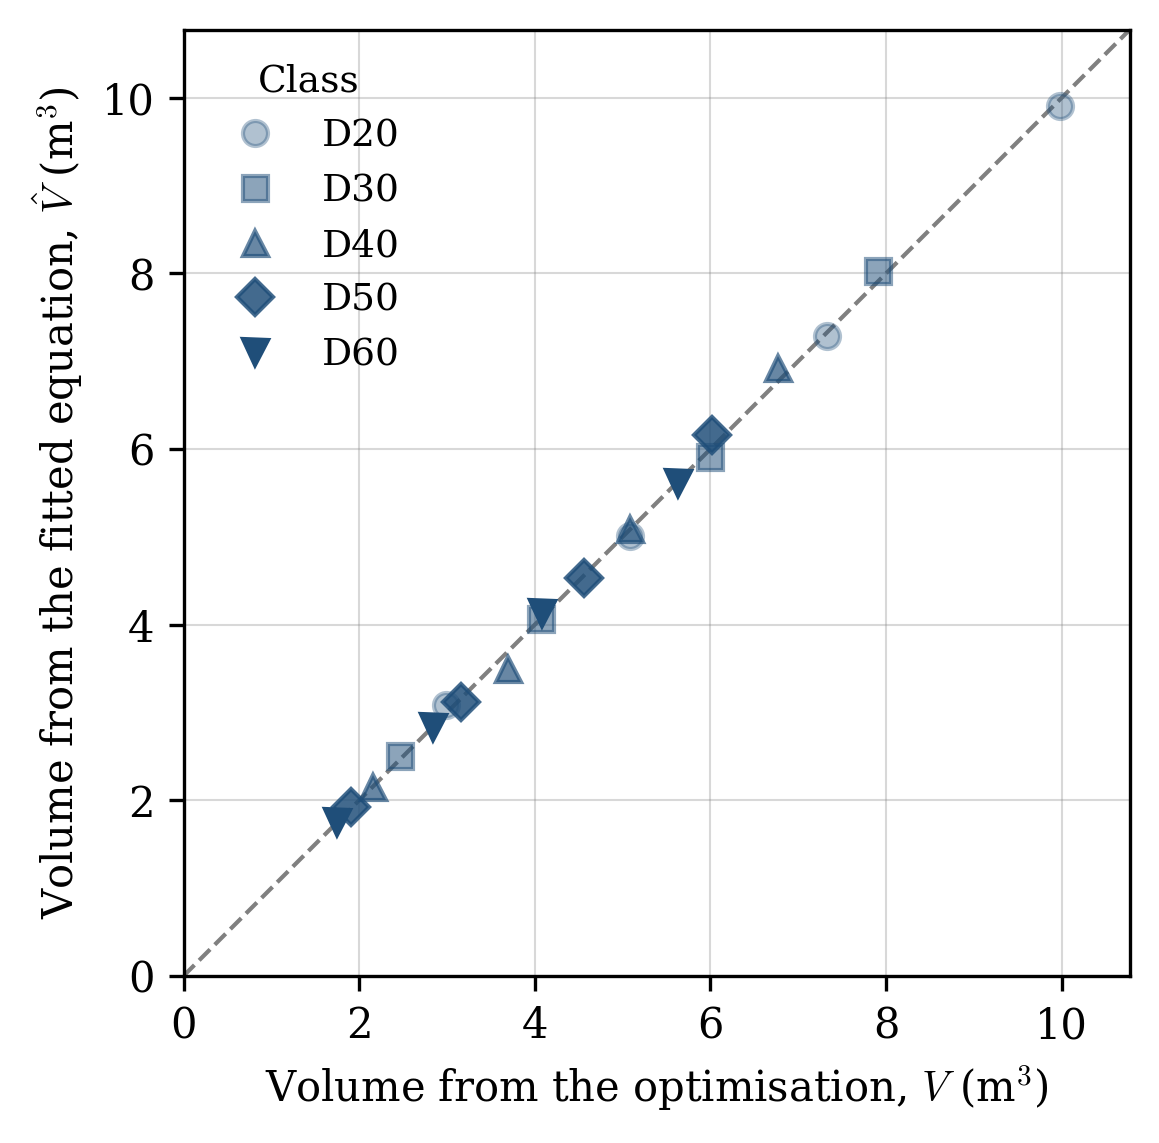
\includegraphics[width=0.4\textwidth]{figuras/en/equacao_pre_dimensionamento.png}
    \caption{Volume estimado pela equação de pré-dimensionamento (Equação~\ref{eq:pre_dimensionamento}) contra o volume obtido na otimização, para as vinte células da matriz.}
    \label{fig:equacao_pre_dimensionamento}
\end{figure}

O erro não se concentra em nenhum subconjunto identificável da matriz: como a Seção~\ref{sec:varredura} mostrou que nenhuma das vinte células satura no piso dimensional do domínio de busca, a Equação~\eqref{eq:pre_dimensionamento} não sofre aqui a limitação, comum a ajustes desse tipo, de ignorar uma restrição lateral do algoritmo: os 5{,}32\% de erro máximo, na célula C-08, refletem apenas o resíduo esperado de um ajuste de três parâmetros sobre vinte observações, sem relação discernível com o vão ou a classe da célula.
Os sinais dos expoentes ajustados têm leitura física direta e reforçam a consistência do modelo com a Seção~\ref{sec:varredura}: $b = 1{,}683 > 1$ reproduz a mesma realimentação entre peso próprio e seção que ali produz expoentes $n$ entre 1{,}64 e 1{,}73 por classe, e $c = -0{,}518 < 0$ expressa que o aumento de $f_{c0,k}$ reduz o volume necessário, como esperado.
O expoente $b$ da equação conjunta situa-se, de fato, dentro da própria faixa de expoentes $n$ observada classe a classe, o que indica que amarrar as cinco curvas por uma única superfície contínua em $f_{c0,k}$ não distorce o comportamento já identificado em cada classe isoladamente.